\documentclass[letter,11pt]{article}

\usepackage[spanish,es-nodecimaldot]{babel}
\usepackage[utf8]{inputenc}

\usepackage{lmodern}
\usepackage[T1]{fontenc}
\usepackage{textcomp}

\usepackage{framed}
\usepackage[svgnames]{xcolor}
\colorlet{shadecolor}{Gainsboro!50}

\usepackage[labelfont=bf]{caption}
\usepackage{graphicx}
\usepackage{pstricks}

\usepackage{anysize}
\marginsize{3cm}{2cm}{2cm}{3cm}

\usepackage{siunitx}
\usepackage{amsmath}
\usepackage{array}
\usepackage{csquotes}
\usepackage{steinmetz}
\usepackage{stmaryrd}
\usepackage{multirow}

\usepackage{fancyhdr}
\usepackage{lastpage}
\pagestyle{fancy}
\fancyhf{}
\fancyhead[LE,RO]{Laboratorio de Circuitos Eléctricos III}
\fancyfoot[CO,CE]{\thepage\ de \pageref{LastPage}}

\special{papersize=215.9mm,279.4mm}

\usepackage[
    pdfauthor={Carlos Eduardo Caballero Burgoa},%
    pdftitle={Laboratorio de Circuitos Eléctricos III},%
    pdfsubject={Medida del factor de potencia trifásico},%
    colorlinks,%
    citecolor=black,%
    filecolor=black,%
    linkcolor=black,%
    urlcolor=black,
    breaklinks]{hyperref}
\usepackage{breakurl}

\renewcommand{\arraystretch}{1.2}

\begin{document}

\begin{titlepage}
    \begin{center}
        {\Large UNIVERSIDAD MAYOR DE SAN SIMÓN}\\
        \vspace*{0.15cm}
        {\large FACULTAD DE CIENCIAS Y TECNOLOGÍA}\\
        \vspace*{0.10cm}
        DEPARTAMENTO DE ELÉCTRICA-ELECTRÓNICA\\
        \vspace*{3.0cm}
        {\Large \textbf{LABORATORIO DE CIRCUITOS ELÉCTRICOS III}}\\
        \vspace*{0.3cm}
        {\Large \textbf{INFORME No. 7}}\\
        \vspace*{3.5cm}
        {\Large \textbf{MEDIDA DEL FACTOR DE POTENCIA TRIFÁSICO}}\\
    \end{center}

    \vspace*{5.3cm}
    \leftskip=7.95cm
    \noindent
    \textbf{Estudiante:}\\
    Caballero Burgoa, Carlos Eduardo.\\
    \newline
    \textbf{Carrera:}\\
    Ing. Electromecánica.\\
    \newline
    \textbf{Docente:}\\
    Ing. Marco Antonio Vallejo Camacho.\\
    \newline
    \textbf{Grupo:} 2F (Martes).\\
\textbf{Fecha de entrega:} 5 de Noviembre del 2024.\\
\end{titlepage}

\section{Cálculos teóricos}

\subsection{Carga $RL$}
\begin{figure}[!h]
\centering
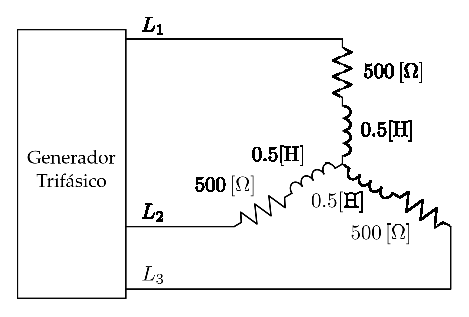
\includegraphics[scale=0.95]{figura1.eps}
\caption{Circuito trifásico equilibrado con carga $RL$.}
\label{circuito1}
\end{figure}

Considerando un circuito trifásico con carga $RL$ estrella equilibrado
(\textbf{Figura~\ref{circuito1}}).

Se calcula la frecuencia angular ($\omega$):
\begin{equation*}
    \begin{split}
        \omega&=2\pi f\\
              &=2\pi(50)\\
              &=100\pi\,[\text{rad}/\text{s}]\\
    \end{split}
\end{equation*}

Se halla la impedancia en el dominio de frecuencia:
\begin{equation*}
    \begin{split}
        Z &= R+j\omega L\\
          &= 500+j\,(100\pi)\,(0.5)\\
          &= 500+j50\pi\,[\Omega]\\
    \end{split}
\end{equation*}

Y su representación fasorial:
\begin{equation*}
    \begin{split}
        |Z| &= \sqrt{500^2+(50\pi)^2}\\
            &= 524.09\\
        \theta &= \arctan\left(\frac{50\pi}{500}\right)\\
               &= 17.44^{\circ}\\
        Z &= 524.09\phase{17.44^{\circ}}\,[\Omega]\\
    \end{split}
\end{equation*}

Por tanto, el factor de potencia es:
\begin{equation*}
    \begin{split}
        \text{fp} &= \cos(17.44^{\circ})\\
                  &= 0.9540\,\text{(atrasado)}\\
    \end{split}
\end{equation*}

\subsection{Carga $RC$}
\begin{figure}[!h]
\centering
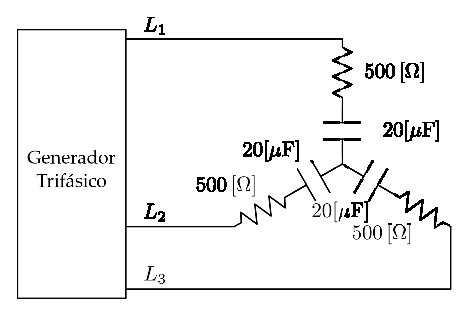
\includegraphics[scale=0.95]{figura2.eps}
\caption{Circuito trifásico equilibrado con carga $RC$.}
\label{circuito2}
\end{figure}

Considerando un circuito trifásico con carga $RC$ estrella equilibrado
(\textbf{Figura~\ref{circuito2}}).

Se halla la impedancia en el dominio de frecuencia:
\begin{equation*}
    \begin{split}
        Z &= R+\frac{1}{j\omega C}\\
          &= 500+\frac{1}{j\,(100\pi)\,(\num{20e-6})}\\
          &= 500-j\frac{500}{\pi}\,[\Omega]\\
    \end{split}
\end{equation*}

Y su representación fasorial:
\begin{equation*}
    \begin{split}
        |Z| &= \sqrt{500^2+\left(-\frac{500}{\pi}\right)^2}\\
            &= 524.72\\
        \theta &= \arctan\left(\frac{-500/\pi}{500}\right)\\
               &= -17.66^{\circ}\\
        Z &= 524.72\phase{-17.66^{\circ}}\,[\Omega]\\
    \end{split}
\end{equation*}

Por tanto, el factor de potencia es:
\begin{equation*}
    \begin{split}
        \text{fp} &= \cos(-17.66^{\circ})\\
                  &= 0.9529\,\text{(adelantado)}\\
    \end{split}
\end{equation*}

\subsection{Resumen de resultados}
En la siguiente tabla se resumen los valores obtenidos teóricamente:

\begin{center}
    \begin{tabular}{|c||c|c|}
    \hline
    & \textbf{Carga $RL$} & \textbf{Carga $RC$}
    \tabularnewline \hline \hline
    $FP$ &
    $0.9540\,\text{(atrasado)}$ &
    $0.9529\,\text{(adelantado)}$
    \tabularnewline \hline
    $\phi\,[^{\circ}]$ &
    $17.44$ &
    $-17.66$
    \tabularnewline \hline
    \end{tabular}
\end{center}

\section{Simulación}
Se utilizó el software \emph{Electronic Workbench v5.12.} para simular
los circuitos, la carga $RL$ puede verse en la
\textbf{Figura~\ref{simulacion1}}, y la carga $RC$ puede verse en la
\textbf{Figura~\ref{simulacion2}}.

\begin{figure}[!h]
\centering
\includegraphics[scale=1.06]{simulacion/practica7.1.eps}
\caption{Simulación de la carga $RL$.}
\label{simulacion1}
\end{figure}

\begin{figure}[!h]
\centering
\includegraphics[scale=1.06]{simulacion/practica7.2.eps}
\caption{Simulación de la carga $RC$.}
\label{simulacion2}
\end{figure}

\subsection{Resumen de resultados}
En la siguiente tabla se resumen los valores obtenidos de la simulación: 
\begin{center}
    \begin{tabular}{|c||c|c|c||c|c|c|}
    \hline
    \multirow{2}{*}{} &
    \multicolumn{3}{|c||}{\textbf{Carga $RL$}} &
    \multicolumn{3}{|c|}{\textbf{Carga $RC$}}\\
    & $Z_1$ & $Z_2$ & $Z_3$ & $Z_1$ & $Z_2$ & $Z_3$\\
    \hline \hline
    $U_{\text{FASE}}\,[\text{V}]$ &
    $220$ &
    $220$ &
    $220$ &
    $220$ &
    $220$ &
    $220$
    \tabularnewline \hline
    $U_R\,[\text{V}]$ &
    $209.7$ &
    $209.6$ &
    $209.6$ &
    $209.8$ &
    $209.9$ &
    $209.9$
    \tabularnewline \hline
    $\text{FP} = U_R/U_{\text{FASE}}$ &
    $0.9532$ &
    $0.9527$ &
    $0.9527$ &
    $0.9536$ &
    $0.9541$ &
    $0.9541$
    \tabularnewline \hline
    $\phi = \cos^{-1}(FP)\,[^{\circ}]$ &
    $17.602$ &
    $17.688$ &
    $17.688$ &
    $-17.515$ &
    $-17.429$ &
    $-17.429$
    \tabularnewline \hline \hline
    \textbf{FP trifásica (promedio)} &
    \multicolumn{3}{|c||}{$0.9529\,\text{(atrasado)}$} &
    \multicolumn{3}{|c|}{$0.9539\,\text{(adelantado)}$}
    \tabularnewline \hline
    \end{tabular}
\end{center}

\section{Tablas y mediciones}
Se presentan los resultados obtenidos con las mediciones de voltaje realizadas
en laboratorio, el calculo del factor de potencia, el ángulo y el factor de
potencia promedio:
\begin{center}
    \begin{tabular}{|c||c|c|c||c|c|c|}
    \hline
    \multirow{2}{*}{} &
    \multicolumn{3}{|c||}{\textbf{Carga $RL$}} &
    \multicolumn{3}{|c|}{\textbf{Carga $RC$}}\\
    & $Z_1$ & $Z_2$ & $Z_3$ & $Z_1$ & $Z_2$ & $Z_3$\\
    \hline \hline
    $U_{\text{FASE}}\,[\text{V}]$ &
    $222$ &
    $221$ &
    $223$ &
    $222$ &
    $222$ &
    $223$
    \tabularnewline \hline
    $U_R\,[\text{V}]$ &
    $209$ &
    $208$ &
    $209$ &
    $211$ &
    $211$ &
    $212$
    \tabularnewline \hline
    $\text{FP} = U_R/U_{\text{FASE}}$ &
    $0.9414$ &
    $0.9412$ &
    $0.9372$ &
    $0.9505$ &
    $0.9505$ &
    $0.9507$
    \tabularnewline \hline
    $\phi = \cos^{-1}(FP)\,[^{\circ}]$ &
    $19.705$ &
    $19.750$ &
    $20.410$ &
    $-18.112$ &
    $-18.112$ &
    $-18.071$
    \tabularnewline \hline \hline
    \textbf{FP trifásica (promedio)} &
    \multicolumn{3}{|c||}{$0.9399\,\text{(atrasado)}$} &
    \multicolumn{3}{|c|}{$0.9505\,\text{(adelantado)}$}
    \tabularnewline \hline
    \end{tabular}
\end{center}
\vspace{0.6cm}

Se presentan los resultados obtenidos con las mediciones realizadas con el
cosímetro para el calculo del factor de potencia, el ángulo y el factor de
potencia promedio:
\begin{center}
    \begin{tabular}{|c||c|c|c||c|c|c|}
    \hline
    \multirow{2}{*}{} &
    \multicolumn{3}{|c||}{\textbf{Carga $RL$}} &
    \multicolumn{3}{|c|}{\textbf{Carga $RC$}}\\
    & $Z_1$ & $Z_2$ & $Z_3$ & $Z_1$ & $Z_2$ & $Z_3$\\
    \hline \hline
    $\text{FP}$ &
    $0.95$ &
    $0.96$ &
    $0.95$ &
    $0.94$ &
    $0.94$ &
    $0.94$
    \tabularnewline \hline
    $\phi\,[^{\circ}]$ &
    $18$ &
    $16$ &
    $18$ &
    $-19$ &
    $-19$ &
    $-19$
    \tabularnewline \hline \hline
    \textbf{FP trifásica (promedio)} &
    \multicolumn{3}{|c||}{$0.9533\,\text{(atrasado)}$} &
    \multicolumn{3}{|c|}{$0.94\,\text{(adelantado)}$}
    \tabularnewline \hline
    \end{tabular}
\end{center}

\section{Cuestionario}

\begin{enumerate}

\item \textbf{A qué se deben las variaciones de factores de potencia entre los
cálculos teóricos y medidos si existen?}

La desviación estándar de los valores del factor de potencia se resumen en la
siguiente tabla:
\begin{center}
    \begin{tabular}{|c||c|c|c||c|c|c|}
    \hline
    \multirow{2}{*}{} &
    \multicolumn{3}{|c||}{\textbf{Carga $RL$}} &
    \multicolumn{3}{|c|}{\textbf{Carga $RC$}}\\
        & $x$ & $x_i-\bar{x}$ & $(x_i-\bar{x})^2$
        & $x$ & $x_i-\bar{x}$ & $(x_i-\bar{x})^2$\\
    \hline \hline
    $Z_1$ &
    $0.9414$ &
    $\num{1.4956e-3}$ &
    $\num{2.2367e-6}$ &
    $0.9505$ &
    $\num{-7.4065e-5}$ &
    $\num{5.4856e-9}$
    \tabularnewline \hline
    $Z_2$ &
    $0.9412$ &
    $\num{1.2306e-3}$ &
    $\num{1.5144e-6}$ &
    $0.9505$ &
    $\num{-7.4065e-5}$ &
    $\num{5.4856e-9}$
    \tabularnewline \hline
    $Z_3$ &
    $0.9372$ &
    $\num{-2.7262e-3}$ &
    $\num{7.4319e-6}$ &
    $0.9507$ &
    $\num{1.4813e-4}$ &
    $\num{2.1943e-8}$
    \tabularnewline \hline \hline
        & \multicolumn{3}{|c||}{$\bar{x} = 0.9399$}
        & \multicolumn{3}{|c|}{$\bar{x} = 0.9506$}
    \tabularnewline \hline
        & \multicolumn{3}{|c||}{$\sigma_{n-1} = \num{2.3646e-3}$}
        & \multicolumn{3}{|c|}{$\sigma_{n-1} = \num{1.2828e-4}$}
    \tabularnewline \hline
    \end{tabular}
\end{center}

Los valores de desviación estándar son muy próximos a cero, lo que implica que
la variación entre los valores se debe a diferencias entre los voltajes de
linea, las resistencias, los inductores y los capacitores.

\item \textbf{Qué otra manera se podría aplicar para medir el factor de potencia
para cada fase?}

Otro modo de medición del factor de potencia puede encontrarse a partir de la
definición de factor de potencia:

\begin{equation*}
    \text{FP} = \frac{P}{|\bar{S}|}
\end{equation*}

Donde:
\begin{itemize}
    \item \textbf{$P$} es la potencia activa consumida por la parte resistiva de
        la impedancia.
    \item \textbf{$|\bar{S}|$}, es la potencia aparente, es decir, la magnitud
        de la potencia compleja.
\end{itemize}

Por tanto midiendo ambas potencias con un vatímetro puede hallarse el factor de
potencia.

\end{enumerate}

\end{document}

